\chapter{Inverse Functions}

\section{Finding the Inverse of a Function}

When finding the inverse of a function, 

\begin{enumerate}
    \item Write $y =$ instead of $f(x) = $.
    \item Switch $x$ and $y$ variables.
    \item Solve the new equation for $y$.
\end{enumerate}

\begin{example}
Determine the inverse of each.
\begin{multicols}{4}
    \begin{enumerate}[(a)]
        \item $f(x) = \tfrac{3}{x-5}$    \label{1a}
        \item $g(x) = \tfrac{6x}{x+1}$   \label{1b}
        \item $h(x) = \sqrt{2x-1}+7$
        \item $j(x) = x^2 - 5x$
    \end{enumerate}
\end{multicols}
\end{example}

\begin{solution}

(a) First, write the function as $y = \tfrac{3}{x-5}$ \newline\\

Next, switch the $x$ and $y$ variables. 
\[
x = \tfrac{3}{y-5}
\]

Now, solve the equation for $y$:

\begin{align*}
    x &= \tfrac{3}{\redy - 5} \\
    x(\redy - 5) &= 3 \qquad \text{Multiply both side by denominator to eliminate fraction} \\
    \redy - 5 &= \tfrac{3}{x} \qquad \text{Divide both sides by $x$ to eliminate need for parentheses} \\
    \redy &= \tfrac{3}{x} + 5 \qquad \text{Add 5 to both sides} 
\end{align*}

The inverse of $f(x)$ is $\boxed{f^{-1}(x) = \tfrac{3}{x} + 5}$ 

\vspace{0.25in}

(b) Writing $g(x) = \tfrac{6x}{x+1}$ as $y = \tfrac{6x}{x+1}$.

\begin{align*} 
    y &= \tfrac{6x}{x+1} \\
    x &= \tfrac{6\redy}{\redy+1} \qquad \text{Switch $x$ and $y$} \\
    x(\redy+1) &= 6\redy \qquad \text{Multiply both sides by denominator to eliminate fraction} \\
    x\redy + x &= 6\redy \qquad \text{Distribute the $x$} \\
    x &= 6\redy - x\redy \qquad \text{Gather $\redy$ terms on one side} \\
    x &= (6-x)\redy \qquad \text{Factor out $\redy$ as greatest common factor} \\
    \tfrac{x}{6-x} &= \redy \qquad \text{Divide both sides by $6-x$} 
\end{align*}

The inverse of $g(x)$ is $\boxed{g^{-1}(x) = \tfrac{x}{6-x}}$ \newline\\

\dotfill \newline

You may have noticed two different strategies for isolating the $\redy$ in the previous two examples. \newline

In Example 1\ref{1a}, there wasn't an $x$ in the numerator. However, in Example 1\ref{1b}, there was. \newline 

For the record, here is what you would do if you decided to divide both sides by $x$ in Example 1\ref{1b} instead of distributing it:

\begin{align*}
    x(\redy+1) &= 6\redy \\
    \redy + 1 &= \tfrac{6\redy}{x} \qquad \text{Divide both sides by $x$} \\
    1 &= \tfrac{6\redy}{x}-\redy \qquad \text{Get $\redy$ terms on one side} \\
    1 &= \left(\tfrac{6}{x}-1\right)\redy \qquad \text{Factor out $\redy$ as greatest common factor} \\
    \tfrac{1}{\tfrac{6}{x}-1} &= \redy \qquad \text{Divide both sides by $\tfrac{6}{x}-1$} \\
    \tfrac{1 \cdot {\color{blue}{x}}}{{\color{blue}{x}} \cdot \tfrac{6}{x}-1 \cdot {\color{blue}{x}}} &= \redy \qquad \text{Multiply every term by least common tiny denominator $x$} \\
    \tfrac{x}{6-x} &= \redy \qquad \text{Simplify} 
\end{align*}

\vspace{11pt}

You get the same answer. However, there is more work involved. \newline 

\dotfill \newline 

(c) For $h(x) = \sqrt{2x-1}+7$
\begin{align*}
    y &= \sqrt{2x-1}+7 \\
    x &= \sqrt{2\redy-1}+7 \qquad \text{Switch $x$ and $y$} \\
    x-7 &= \sqrt{2\redy-1} \qquad \text{Subtract 7 from both sides} \\
    (x-7)^2 &= 2\redy -1 \qquad \text{Square both sides} \\
    (x-7)^2 + 1 &= 2\redy \qquad \text{Add 1 to both sides} \\
    \tfrac{(x-7)^2+1}{2} &= \redy \qquad \text{Divide both sides by 2}
\end{align*}

The inverse of $h(x)$ is $\boxed{h^{-1}(x) = \tfrac{(x-7)^2+1}{2} \text{ or } \tfrac{1}{2}\left((x-7)^2+1\right)}$

\vspace{0.25in}

(d) For $j(x) = x^2 - 5x$, start by writing it in {\color{-red!75}\textbf{vertex form}}, $y = a(x-h)^2 + k$, where the coordinates of the vertex are $(h, k)$ and $a$ is the coefficient of the $x^2$ term. \newline 

\emph{Note:} Some math teachers call this process \textit{completing the square}.

\[
x^2 - 5x = \left(x-\tfrac{5}{2}\right)^2 - \tfrac{25}{4}
\]

\begin{align*}
    y &= \left(x-\tfrac{5}{2}\right)^2-\tfrac{25}{4} \\
    x &= \left(\redy-\tfrac{5}{2}\right)^2-\tfrac{25}{4} \qquad \text{Switch $x$ and $y$} \\
    x + \tfrac{25}{4} &= \left(\redy-\tfrac{5}{2}\right)^2 \qquad \text{Add $\tfrac{25}{4}$ to both sides} \\
    \pm \sqrt{x + \tfrac{25}{4}} &= \redy - \tfrac{5}{2} \qquad \text{Take the square root of both sides} \\
    \tfrac{5}{2} \pm \sqrt{x + \tfrac{25}{4}} &= \redy \qquad \text{Add $\tfrac{5}{2}$ to both sides}
\end{align*}

The inverse of $j(x)$ is $\boxed{j^{-1}(x) = \tfrac{5}{2} \pm \sqrt{x + \tfrac{25}{4}}}$ \newline\\

or is it ... ? 
\end{solution}

\section{Domains and Ranges of Inverse Functions}

If we look at the graph of $j^{-1}(x) = \tfrac{5}{2} \pm \sqrt{x + \tfrac{25}{4}}$, it actually consists of 2 functons:

\begin{itemize}
    \item $\tfrac{5}{2} + \sqrt{x+\tfrac{25}{4}}$
    \item $\tfrac{5}{2} - \sqrt{x+\tfrac{25}{4}}$
\end{itemize}

The graph of $j^{-1}(x)$, shown below, fails the Vertical Line Test. Thus, it is not a function. \newline 

\emph{Note}: This is also evident from the fact that $j(x) = x^2 - 5x$ fails the Horizontal Line Test. \newline 

\begin{center}
\begin{tikzpicture}
\begin{axis}
[axis lines = middle, xmin = -8, xmax = 2, ymin = -1, ymax = 6]
\addplot [blue, thick, samples = 200, domain=-6.25:2] {2.5 + sqrt(x+6.25)};
\addplot [blue, thick, samples = 200, domain=-6.25:2] {2.5 - sqrt(x+6.25)};
\end{axis}
\end{tikzpicture}
\end{center}

When you switch the $x$ and $y$, you also switch the domains and ranges of the given function and its inverse. \newline 

\begin{center}
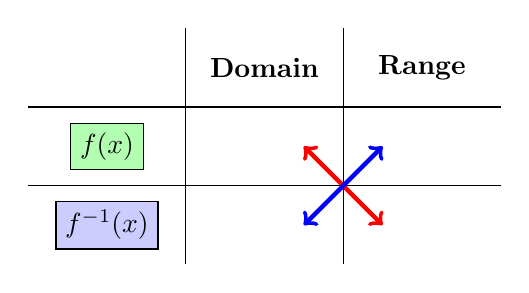
\begin{tikzpicture}
\node [rectangle, draw, fill=green!30] at (0,0.5) {$f(x)$};
\node [rectangle, draw, fill=blue!20] at (0,-0.5) {$f^{-1}(x)$};
\draw (1,-1) -- (1,2);  % creates 1st column
\draw (-1,1) -- (5,1);
\draw (3,-1) -- (3,2);  % creates 2nd column
\node at (2,1.5) {\textbf{Domain}};
\node at (4,1.5) {\textbf{Range}};
\draw (-1,0) -- (5,0);
\draw[<->, ultra thick, red] (2.5,0.5) -- (3.5,-0.5);
\draw[<->, ultra thick, blue] (2.5,-0.5) -- (3.5,0.5);
\end{tikzpicture}
\end{center}

From a visual perspective, switching the $x$ and $y$ also \emph{reflects the given function across the line $y = x$}. \newline 

\begin{center}
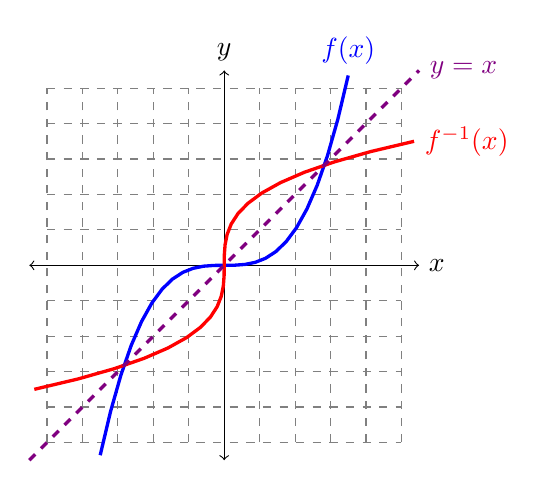
\begin{tikzpicture}[scale=0.45]
\draw [color=gray, dashed] (-5,-5) grid (5,5);
\draw[<->] (-5.5,0) -- (5.5,0) node [right] {$x$};
\draw[<->] (0,-5.5) -- (0,5.5) node [above] {$y$};
\draw [color=blue, very thick, domain=-1.75:1.75, xscale=2] plot (\x, {\x*\x*\x}) node [above] {$f(x)$};
\draw [color=red, very thick, domain=-1.75:1.75, yscale=2] plot ({\x*\x*\x}, \x) node [right] {$f^{-1}(x)$};
\draw [color=violet, very thick, dashed] (-5.5,-5.5) -- (5.5,5.5) node [right] {$y=x$};
\end{tikzpicture}
\end{center}

This is not \emph{just} a result of switching $x$ and $y$, it is a \emph{necessity}.

\begin{quote}
    The graph of a function and the graph of its inverse \textbf{must} be reflections of each other across the line $y = x$.
\end{quote}

This means you may need to restrict the domain and/or range of a function or its inverse in order for this to happen. \newline 

{\color{blue}\textbf{If it is easier, you can also examine the graph of the given function to get a sense of what its domain and range are}}. Then copy the values into the range and domain, respectively, of the inverse function. \newline 

\begin{example}
Determine the domain and range of each function and its inverse.
\begin{multicols}{4}
    \begin{enumerate}[(a)]
        \item $f(x) = \tfrac{3}{x-5}$    
        \item $g(x) = \tfrac{6x}{x+1}$   
        \item $h(x) = \sqrt{2x-1}+7$
        \item $j(x) = x^2 - 5x; \quad x \leq \frac{5}{2}$   \label{2d}
    \end{enumerate}
\end{multicols}
\end{example}

\begin{solution}

(a) For $f(x) = \frac{3}{x-5}$, it might not be easy to get a sense of the domain and range from the graph. However, because of the $x-5$ in the denominator, the domain is $(-\infty, 5) \cup (5, \infty)$. This is also the range of the inverse function, $f^{-1}(x) = \frac{3}{x} + 5$. \newline 

Speaking of $f^{-1}(x) = \frac{3}{x} + 5$, the domain of this inverse function is $(-\infty, 0) \cup (0, \infty)$; which is also the range of the given function $f(x) = \frac{3}{x-5}$. \newline 

Thus, we can fill out the table below as follows. 

\begin{center}
\begin{tabular}{c|c|c}  
     & Domain & Range \\ \hline 
     $f(x)=\frac{3}{x-5}$ & \cellcolor{yellow} $(-\infty, 5) \cup (5, \infty)$ & \cellcolor{green} $(-\infty, 0) \cup (0, \infty)$ \\[4pt] \hline 
     $f^{-1}(x) = \frac{3}{x}+5$ & \cellcolor{green} $(-\infty, 0) \cup (0, \infty)$ & \cellcolor{yellow} $(-\infty, 5) \cup (5, \infty)$ \\[4pt]
\end{tabular}
\end{center}

\vspace{0.25in}

The graphs of $f(x)$ and $f^{-1}(x)$ are shown below, along with the line $y = x$.

\begin{center}
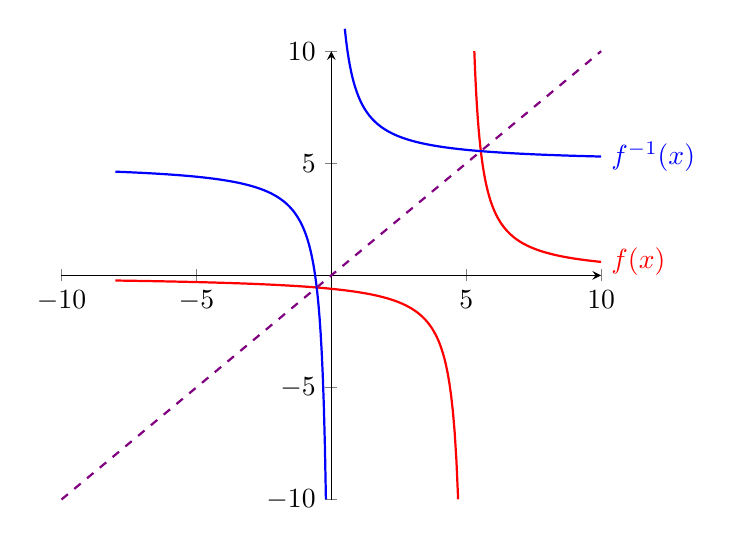
\begin{tikzpicture}
\begin{axis}
    [axis lines = middle, xmin = -10, xmax = 10, ymin = -10, ymax = 10, clip=false]
\addplot [red, thick, samples = 200, domain=-8:4.7] plot {3/(x-5)};
\addplot [red, thick, samples = 200, domain=5.3:10] plot {3/(x-5)} node [right] {$f(x)$};
\addplot [blue, thick, samples = 200, domain=-8:-0.2] plot {5 + (3/x)};
\addplot [blue, thick, samples = 200, domain=0.5:10, label=$f^{-1}(x)$] plot {5 + (3/x)} node [right] {$f^{-1}(x)$};
\addplot [violet, thick, dashed, domain=-10:10] plot {x};
\end{axis}
\end{tikzpicture}
\end{center}

(b) Like part (a), it might not be easy to get a sense of the domain and range by looking at the graph of $g(x) = \frac{6x}{x+1}$. But we can use the $x+1$ in the denominator to get a domain of $(-\infty, -1) \cup (-1, \infty)$. This is also the range of $g^{-1}(x) = \frac{x}{6-x}$. \newline 

The domain of $g^{-1}(x) = \frac{x}{6-x}$ is $(-\infty, 6) \cup (6, \infty)$; which is the range of the given function $g(x)$.

\begin{center}
\begin{tabular}{c|c|c}  
     & Domain & Range \\ \hline 
     $g(x)=\frac{6x}{x+1}$ & \cellcolor{yellow} $(-\infty, -1) \cup (-1, \infty)$ & \cellcolor{green} $(-\infty, 6) \cup (6, \infty)$ \\[4pt] \hline 
     $g^{-1}(x) = \frac{x}{6-x}$ & \cellcolor{green} $(-\infty, 6) \cup (6, \infty)$ & \cellcolor{yellow} $(-\infty, -1) \cup (-1, \infty)$ \\[4pt]
\end{tabular}
\end{center}

\vspace{0.25in}

The graphs of $g(x)$ and $g^{-1}(x)$ are shown below, along with the line $y = x$.

\begin{center}
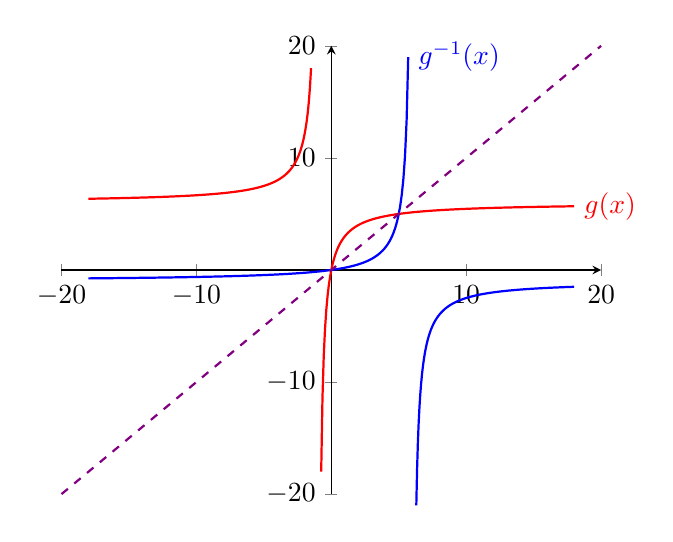
\begin{tikzpicture}
\begin{axis}
    [axis lines = middle, xmin = -20, xmax = 20, ymin = -20, ymax = 20, clip=false]
\addplot [red, thick, samples = 200, domain=-18:-1.5] plot {6*x/(x+1)};
\addplot [red, thick, samples = 200, domain=-0.75:18] plot {6*x/(x+1)} node [right] {$g(x)$};
\addplot [blue, thick, samples = 200, domain=-18:5.7] plot {x/(6-x)} node [right] {$g^{-1}(x)$};
\addplot [blue, thick, samples = 200, domain=6.3:18] plot {x/(6-x)};
\addplot [violet, thick, dashed, domain=-20:20] plot {x};
\end{axis}
\end{tikzpicture}
\end{center}

(c) For $h(x) = \sqrt{2x-1}+7$, since we have $2x-1$ inside of an even root, we need to solve $2x-1 \geq 0$. This gives us $\left[\frac{1}{2}, \infty\right)$. \newline 

Our inverse function, $h^{-1}(x)$, is $h^{-1}(x) = \frac{(x-7)^2+1}{2}$. If we look at the graphs of $h(x)$ and $h^{-1}(x)$, notice they are \underline{not} reflections of each other across the line $y = x$. \newline 

\begin{center}
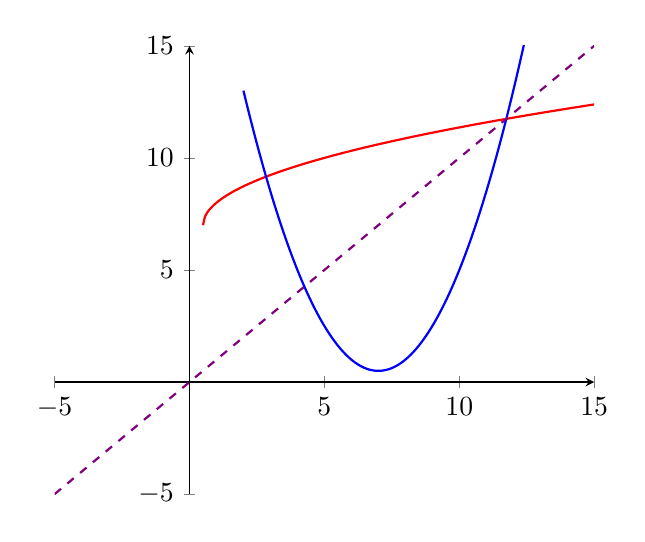
\begin{tikzpicture}
\begin{axis}
    [axis lines = middle, xmin = -5, xmax = 15, ymin = -5, ymax = 15]
    \addplot [red, thick, samples = 200, domain=0.5:15] plot {sqrt(2*x-1)+7};
    \addplot [blue, thick, samples = 200, domain = 2:12.5] plot {0.5*((x-7)^2+1)};
    \addplot [violet, dashed, thick, domain=-5:15] plot {x};
\end{axis}
\end{tikzpicture}
\end{center}

So we need to restrict the domain of the inverse function $h^{-1}(x)$ so that it is a reflection of $h(x) = \sqrt{2x-1}+7$ across the line $y = x$. \newline 

An easy way to know what domain restriction you need to use is to look at the \textbf{range} of the original function $h(x) = \sqrt{2x-1}+7$. \newline 

The lowest $y$-coordinate on the graph is at $\left(\frac{1}{2}, 7\right)$. Notice we can get that $y$-coordinate by evaluating $h(x) = \sqrt{2x-1}+7$ at $x = \frac{1}{2}$. \newline 

Since the $y$-coordinates of $h(x)=\sqrt{2x-1}+7$ increase beyond $y = 7$, the range of $h(x)$ is $[7, \infty)$. \newline 

This must be the domain restriction we use on $h^{-1}(x) = \frac{(x-7)^2+1}{2}$.

\begin{center}
\begin{tabular}{c|c|c}  
     & Domain & Range \\ \hline 
     $h(x)=\sqrt{2x-1}+7$ & \cellcolor{yellow} $\left[\frac{1}{2}, \infty\right)$ & \cellcolor{green} $[7, \infty)$ \\[4pt] \hline 
     $h^{-1}(x) = \frac{(x-7)^2+1}{2}$ & \cellcolor{green} $[7, \infty)$ & \cellcolor{yellow} $\left[\frac{1}{2}, \infty\right)$ \\[4pt]
\end{tabular}
\end{center}

\begin{center}
\begin{tikzpicture}
\begin{axis}
    [axis lines = middle, xmin = -5, xmax = 15, ymin = -5, ymax = 15, clip=false]
    \addplot [red, thick, samples = 200, domain=0.5:15] plot {sqrt(2*x-1)+7} node [right] {$h(x)$};
    \addplot [blue, thick, samples = 200, domain = 7:12.5] plot {0.5*((x-7)^2+1)} node [above] {$h^{-1}(x)$};
    \addplot [violet, dashed, thick, domain=-5:15] plot {x};
\end{axis}
\end{tikzpicture}
\end{center}

\vspace{0.25in}

(d) Earlier, we determined the inverse of $j(x) = x^2 - 5x$ to be either $\frac{5}{2} + \sqrt{x + \frac{25}{4}}$ or $\frac{5}{2} - \sqrt{x + \frac{25}{4}}$. \newline 

With the domain restriction given in Example 2\ref{2d}, $x \leq \frac{5}{2}$, we can graph that piecewise function below:

\begin{center}
\begin{tikzpicture}
\begin{axis}
    [axis lines = middle, xmin = -2, xmax = 6, ymin = -7, ymax = 6]
    \addplot [red, thick, samples=200, domain=-1.5:2.5] plot {x^2-5*x};
\end{axis}
\end{tikzpicture}
\end{center}

Notice the domain of the graph above is $\left(-\infty, \frac{5}{2}\right]$. \newline 

If we compare $y = \frac{5}{2} + \sqrt{x + \frac{25}{4}}$ and $y = \frac{5}{2} - \sqrt{x + \frac{25}{4}}$, the graph of $y = \frac{5}{2} - \sqrt{x + \frac{25}{4}}$ has a  \underline{range} of $\left(-\infty, \frac{5}{2}\right]$.

\begin{center}
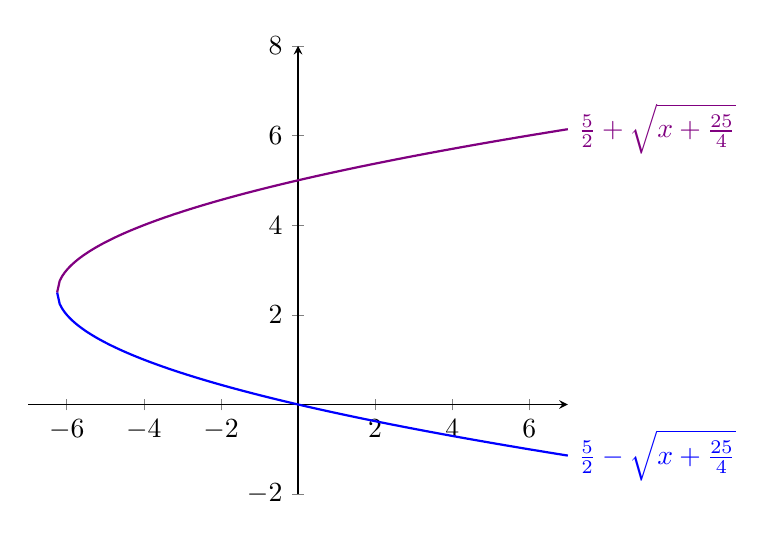
\begin{tikzpicture}
\begin{axis}
    [axis lines = middle, xmin = -7, xmax=7, ymin=-2, ymax=8, clip=false]
    \addplot [blue, thick, samples = 200, domain = -6.25:7] plot {2.5-sqrt(x+6.25)} node [right] {$\frac{5}{2}-\sqrt{x+\frac{25}{4}}$};
    \addplot [violet, thick, samples = 200, domain = -6.25:7] plot {2.5+sqrt(x+6.25)} node [right] {$\frac{5}{2}+\sqrt{x+\frac{25}{4}}$};
\end{axis}
\end{tikzpicture}
\end{center}

Thus, the inverse of $j(x) = x^2 - 5x; \, x \leq \frac{5}{2}$ is $\boxed{j^{-1}(x) = \tfrac{5}{2}-\sqrt{x+\tfrac{25}{4}}}$.

Also, note that the graph of $\frac{5}{2}-\sqrt{x+\frac{25}{4}}$ is the reflection of the piecewise function $x^2 - 5x; \, x \leq \frac{5}{2}$ across the line $y = x$.

\begin{center}
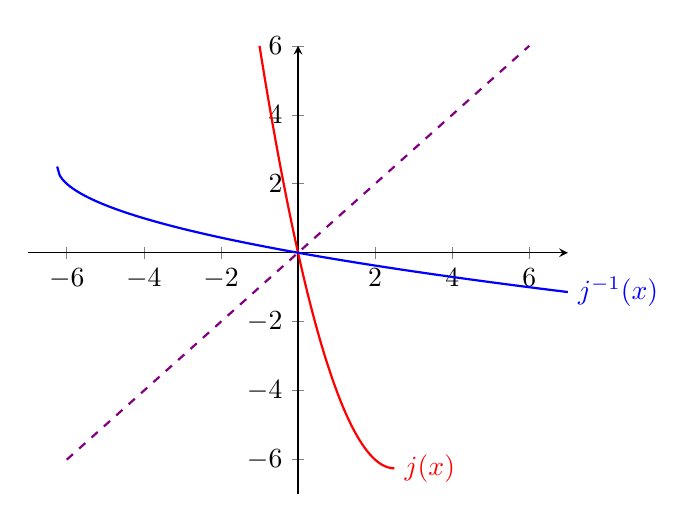
\begin{tikzpicture}
\begin{axis}
    [axis lines = middle, xmin = -7, xmax=7, ymin=-7, ymax=6, clip=false]
    \addplot [red, thick, samples = 200, domain = -1:2.5] plot {x^2-5*x} node [right] {$j(x)$};
    \addplot [blue, thick, samples = 200, domain = -6.25:7] plot {2.5-sqrt(x+6.25)} node [right] {$j^{-1}(x)$};
    \addplot [violet, thick, dashed, domain=-6:6] plot {x};
\end{axis}
\end{tikzpicture}
\end{center}

\vspace{0.25in}

To find the range of our starting function, $j(x)$, we can either look at $y$-coordinates on the graph of $j(x)$ or find the domain of $j^{-1}(x) = \frac{5}{2} - \sqrt{x + \frac{25}{4}}$ \newline 

In any event, we can find that the range of $j(x)$ [or, equally, the domain of $j^{-1}(x)$] is $x \geq -\frac{25}{4}$.

\begin{center}
\begin{tabular}{c|c|c}  
     & Domain & Range \\ \hline 
     $j(x)=x^2-5x$ & \cellcolor{yellow} $\left(-\infty, \frac{5}{2}\right]$ & \cellcolor{green} $\left[-\frac{25}{4}, \infty\right)$ \\[4pt] \hline 
     $j^{-1}(x) = \frac{(x-7)^2+1}{2}$ & \cellcolor{green} $\left[-\frac{25}{4}, \infty\right)$ & \cellcolor{yellow} $\left(-\infty, \frac{5}{2}\right]$ \\[4pt]
\end{tabular}
\end{center}

\end{solution}

\section{Exercises}

Find the inverse of each. Then state the domain and range of the function and the inverse.

\begin{enumerate}
	\item $f(x) = \sqrt{-2x + 3} + 1$
	\item $g(x) = (x+4)^2 - 1, \, x \leq -4$
	\item $h(x) = \frac{9x}{4x-1}$
	\item $f(x) = \sqrt{x} - 3$
	\item $g(x) = \frac{1}{1-x}$
	\item $h(x) = x^2 + 6x + 4, \, x \leq -3$
	\item $f(x) = \sqrt{5x-4}$
	\item $g(x) = x^2 - 2x + 3, \, x \leq 1$
	\item $h(x) = \frac{3}{x-1}$
	
	\item $f(x) = 5-\sqrt{2x}$
    \item $g(x) = \frac{5}{x+1}$
    \item $h(x) = \frac{3x}{x-2}$
\end{enumerate}

\newpage

\section{Answer Key}

\begin{enumerate}	\setlength{\itemsep}{15pt}
	\item $f^{-1}(x) = -\frac{1}{2}\left((x-1)^2-3\right)$ \newline\\
     \begin{tabular}{c|c|c}
         &   Domain  &   Range   \\  \hline
         $f(x)$ & $(-\infty, 1.5]$ & $[1, \infty)$ \\ \hline
         $f^{-1}(x)$ & $[1, \infty)$ & $(-\infty, 1.5]$ \\ 
     \end{tabular}
     
     \item $g^{-1}(x) = -\sqrt{x+1}-4$   \newline\\
     \begin{tabular}{c|c|c}
         &   Domain  &   Range   \\  \hline
         $g(x)$ & $(-\infty, -4]$ & $[-1, \infty)$ \\ \hline
         $g^{-1}(x)$ & $[-1, \infty)$ & $(-\infty, -4]$ \\ 
     \end{tabular}
     
     \item $h^{-1}(x) = \frac{-x}{9-4x}$ \newline\\
     \begin{tabular}{c|c|c}
         &   Domain  &   Range   \\  \hline
         $h(x)$ & $(-\infty, 1/4) \cup (1/4, \infty) $ & $(\infty, 9/4) \cup (9/4, \infty)$ \\ \hline
         $h^{-1}(x)$ & $(\infty, 9/4) \cup (9/4, \infty)$ & $(-\infty, 1/4) \cup (1/4, \infty) $ \\ 
     \end{tabular}
         
     \item $f^{-1}(x) = (x+3)^2$ \newline\\
	\begin{tabular}{c|c|c}
            &   Dom             &   Ran \\  \hline
    $f(x)$  &   $[0,\infty)$    &   $[-3,\infty)$   \\  \hline
    $f^{-1}(x)$ &   $[-3,\infty)$   &   $[0,\infty)$    \\
\end{tabular}
     
     \item $g^{-1}(x) = 1 - \frac{1}{x}$  \newline\\
\begin{tabular}{c|c|c}
            &   Dom             &   Ran \\  \hline
    $g(x)$  &   $(-\infty,1)\cup(1,\infty)$    &   $(-\infty,0)\cup(0,\infty)$   \\  \hline
    $g^{-1}(x)$ &   $(-\infty,0)\cup(0,\infty)$   &   $(-\infty,1)\cup(1,\infty)$    \\
\end{tabular}

\item $h^{-1}(x) = -\sqrt{x+5}-3$ \newline\\ 
\begin{tabular}{c|c|c}
            &   Dom             &   Ran \\  \hline
    $h(x)$  &   $(-\infty,-3]$    &   $[-5,\infty)$   \\  \hline
    $h^{-1}(x)$ &   $[-5,\infty)$   &   $(-\infty,-3]$    \\
\end{tabular}

\item $f^{-1}(x) = \frac{1}{5}x^2 + \frac{4}{5}$    \newline\\
    \setlength{\extrarowheight}{5pt}
    \begin{tabular}{c|c|c}
            &   Dom &   Ran \\  \hline
        $f(x)$  &   $\left[\frac{4}{5}, \infty\right)$  &   $[0, \infty)$    \\ \hline
        $f^{-1}(x)$ &   $[0, \infty)$   &   $\left[\frac{4}{5}, \infty\right)$  \\
    \end{tabular}
    
\item $g^{-1}(x) = -\sqrt{x-2}+1$   \newline\\
    \begin{tabular}{c|c|c}
            &   Dom &   Ran \\  \hline
        $g(x)$  &   $(-\infty, 1]$  &   $[2, \infty)$    \\  \hline
        $g^{-1}(x)$ &   $[2, \infty)$   &   $(-\infty, 1]$  \\
    \end{tabular}
    
\item $h^{-1}(x) = \frac{3}{x} + 1$ \newline\\
    \begin{tabular}{c|c|c}
            &   Dom &   Ran \\  \hline
        $h(x)$  &   $(-\infty, 1) \cup (1, \infty)$  &   $(-\infty, 0) \cup (0, \infty)$    \\[5pt]  \hline
        $h^{-1}(x)$ &   $(-\infty, 0) \cup (0, \infty)$   &   $(-\infty, 1) \cup (1, \infty)$  \\
        \end{tabular}
        
\item $f^{-1}(x) = \frac{1}{2}(x-5)^2; \, x \leq 5$ \newline\\
    
    \begin{tabular}{c|c|c}
                    &   Domain      & Range             \\ \hline
        $f(x)$      & $[0,\infty)$  &   $(-\infty, 5]$  \\  \hline   
        $f^{-1}(x)$ & $(-\infty,5]$ &   $[0,\infty)$  
    \end{tabular}
    
    \item $g^{-1}(x) = \frac{5}{x}-1$   \newline\\
    
    \begin{tabular}{c|c|c}
                    &   Domain      & Range             \\ \hline
        $g(x)$      & $(-\infty,-1)\cup(-1,\infty)$  &   $(-\infty,0)\cup(0,\infty)$  \\  \hline   
        $g^{-1}(x)$ & $(-\infty,0)\cup(0,\infty)$ &   $(-\infty,-1)\cup(-1,\infty)$  
    \end{tabular}
    
    \item $h^{-1}(x) = \frac{2x}{x-3}$    \newline\\
    
    \begin{tabular}{c|c|c}
                    &   Domain      & Range             \\ \hline
        $h(x)$      & $(-\infty,2)\cup(2,\infty)$  &   $(-\infty,3)\cup(3,\infty)$  \\  \hline   
        $h^{-1}(x)$ & $(-\infty,3)\cup(3,\infty)$ &   $(-\infty,2)\cup(2,\infty)$  
    \end{tabular}

    



\end{enumerate}